\documentclass[presentation,10pt]{beamer}
%\documentclass[hyperref=unicode, handout,10pt]{beamer}
%\usepackage{handoutWithNotes}

\mode<presentation>{\usetheme{default}
 \usecolortheme{crane}}

\usepackage[absolute,overlay]{textpos}
\usepackage{array}
\usepackage{graphicx}
\usepackage{adjustbox}
\usepackage[version=3]{mhchem}
\usepackage{chemfig}
\usepackage{textcomp}
\usepackage{ucs}
\usepackage[utf8]{inputenc}

\usepackage{multirow}

\PrerenderUnicode{ěščřžýáíéĚŠČŘŽÝÁÍÉďťňĎŤŇůúÚóÓ}

\usepackage[czech]{babel}

\setbeamertemplate{footline}[frame number]

\addtobeamertemplate{frametitle}{
   \let\insertframetitle\insertsectionhead}{}
\addtobeamertemplate{frametitle}{
   \let\insertframesubtitle\insertsubsectionhead}{}

\makeatletter
  \CheckCommand*\beamer@checkframetitle{\@ifnextchar\bgroup\beamer@inlineframetitle{}}
  \renewcommand*\beamer@checkframetitle{\global\let\beamer@frametitle\relax\@ifnextchar\bgroup\beamer@inlineframetitle{}}
\makeatother
\setbeamercolor{section in toc}{fg=blue}
\setbeamertemplate{section in toc shaded}[default][100]

\begin{document}
\title[Crisis] % (optional, only for long titles)
{Vyhodnocování IR a RA spekter}

\author % (optional, for multiple authors)
{Zdeněk Moravec, Ústav chemie, PřF MU \\ hugo@chemi.muni.cz \\
\includegraphics[width=85mm]{img/raman-spect.png}}
%{http://z-moravec.net}

\date{ } %hide date on titlepage

%\subtitle{Metody chemické výzkumu}

\frame{\titlepage}

\section{Osnova}
\frame{
	\frametitle{}
	\vfill
	\tableofcontents
	\iffalse
	\begin{itemize}
	\item Úvod
	\item Charakteristické frekvence
	\item Vliv vodíkových vazeb
	\item Spektra izotopicky substituovaných molekul
	\item Databáze spekter
	\item Kvantitativní analýza
	\item Coupling TGA/IR
	\item Literatura a odkazy
	\end{itemize}
	\fi
	\vfill
}


\section{Kvalitativní analýza}
\subsection{Rozdělení oblastí spekter}
\frame{
	\frametitle{}
	\vfill
	\begin{itemize}
	\item  NIR (0,7 -- 2,5 $\mu$m; 14 000 - 4 000 cm$^{-1}$) - infračervená spektroskopie v blízké oblasti -- převážně overtony a kombinační vibrace. Intenzita pásů je nižší než v MIR oblasti a pásy se často překrývají.
	\item  \textbf{MIR (2,5 -- 25 $\mu$m; 4 000 - 400 cm$^{-1}$) - infračervená spektroskopie ve střední oblasti} -- základní vibrace molekul.
	\item  FIR (25 -- 1000 $\mu$m; 400 - 10 cm$^{-1}$) - infračervená spektroskopie ve vzdálené oblasti -- vibrace vazeb kov-halogen, deformační vibrace skeletu molekul.
	\end{itemize}
	\vfill
}


\subsection{Důležité oblasti v MIR spektru}
\frame{
	\frametitle{}
	\vfill
	\begin{itemize}
	\item 4000-2500 cm$^{-1}$ oblast valenčních vibrací X-H
	\item 2500-2000 cm$^{-1}$ oblast trojných vazeb
	\item 2000-1500 cm$^{-1}$ oblast dvojných vazeb
	\item 1500-600 cm$^{-1}$ oblast otisku prstu (fingerprint)
	\end{itemize}
	\includegraphics[width=85mm]{img/irBandsOrg.png}
	\vfill
}

\subsection{Charakteristické frekvence}
\frame{
	\frametitle{}
	\vfill
	\adjincludegraphics[width=115mm,valign=l]{img/tab.png}
	\vfill
}

\subsubsection{Organické sloučeniny}
\frame{
	\frametitle{}
	\vfill
	\begin{tabular}{|l|l|l|}
	\hline
	\textbf{Sloučenina} & \textbf{Skupina} & \textbf{Vlnočet [cm$^{-1}$]} \\\hline
	\multirow{2}{*}{Alkany} & \ce{C-H} & 2850-3000 \\ 
	& \ce{C-C} & 800-1000 \\\hline
	\multirow{2}{*}{Aromáty} & \ce{C-H} & 3000-3100 \\ 
	& \ce{C=C} & 1450-1600 \\\hline
	\multirow{2}{*}{Alkeny} & \ce{C-H} & 3080-3140 \\ 
	& \ce{C=C} & 1630-1670 \\\hline
	\multirow{2}{*}{Alkyny} & \ce{C-H} & 3300-3320 \\ 
	& \ce{C\bond{3}C} & 2100-2140 \\\hline
	\multirow{2}{*}{Alkoholy} & \ce{O-H} & 3300-3600 \\ 
	& \ce{C-O} & 1050-1200 \\\hline
	\multirow{2}{*}{Alkyny} & \ce{C-H} & 3300-3320 \\ 
	& \ce{C\bond{3}C} & 2100-2140 \\\hline
	\multirow{2}{*}{Aldehydy} & \ce{C=O} & 1720-1740 \\ 
	& \ce{C-H} & 2700-2900 \\\hline
	\multirow{3}{*}{Karboxylové kyseliny} & \ce{C=O} & 1700-1725 \\ 
	& \ce{O-H} & 2500-3300 \\
	& \ce{C-O} & 1100-1300 \\\hline
	\end{tabular}
	\vfill
}

\subsubsection{Aromatické sloučeniny}
\frame{
	\frametitle{}
	\vfill
	\begin{tabular}{|l|l|}
	\hline
	\textbf{Vibrace} & \textbf{Vlnočet [cm$^{-1}$]} \\\hline
	\ce{C-H} valenční & 3100-3000 \\\hline
	Kombinační, overtony & 2000-1700 \\\hline
	\ce{C=C} & 1650-1430 \\\hline
	\ce{C-H} deformační v rovině kruhu & 1275-1000 \\\hline
	\ce{C-H} deformační mimo rovinu kruhu & 900-690 \\\hline
	\end{tabular}
	\includegraphics[width=85mm]{img/toluene.png}
	\vfill
}

\subsubsection{Halogenované sloučeniny}
\frame{
	\frametitle{}
	\vfill
	\begin{itemize}
	\item Se vzrůstající hmotností halogenu klesá hodnota vlnočtu vazby \ce{C-X}.
	\item V tabulce jsou shrnuty vibrace vazeb \ce{C-X} u alifatických uhlovodíků.
	\end{itemize}
	\begin{tabular}{|l|l|}
	\hline
	\textbf{Vazba} & \textbf{Vlnočet [cm$^{-1}$]} \\\hline
	\ce{C-F} & 1150-1000 \\\hline
	\ce{C-Cl} & 800-700 \\\hline
	\ce{C-Br} & 700-600 \\\hline
	\ce{C-I} & 600-500 \\\hline
	\end{tabular}
	\vfill
}

\subsubsection{Anorganické sloučeniny}
\frame{
	\frametitle{}
	\vfill
	\begin{tabular}{|l|l|}
	\hline
	\textbf{Ion} & \textbf{Vlnočet [cm$^{-1}$]} \\\hline
	\multirow{2}{*}{\ce{CO$_3^{2-}$}} & 1450-1410 \\ 
	& 880-800 \\\hline
	\multirow{2}{*}{\ce{SO$_4^{2-}$}} & 1130-1080 \\ 
	& 680-610 \\\hline
	\multirow{2}{*}{\ce{NO$_3^{-}$}} & 1410-1340 \\ 
	& 860-800 \\\hline
	\ce{PO$_4^{3-}$} & 1100-950 \\\hline
	\ce{SiO$_4^{2-}$} & 1100-900 \\\hline
	\multirow{2}{*}{\ce{NH$_4^{+}$}} & 3335-3030 \\ 
	& 1485-1390 \\\hline
	\multirow{2}{*}{\ce{MnO$_4^{-}$}} & 920-890 \\ 
	& 850-840 \\\hline
	\multirow{2}{*}{\ce{M-H}} & 2250-1700 \\
	& 800-600 \\\hline
	\ce{M-X} & 750-100 \\\hline
	\ce{M=O} & 1010-850 \\\hline
	\ce{M=N} & 1020-875 \\\hline
	\end{tabular}
	\vfill
}

\frame{
	\frametitle{}
	\vfill
	\begin{itemize}
	\item Spektra anorganických sloučenin zpravidla obsahují méně pásů, ty jsou širší a nalézáme je i na nižších vlnočtech, často až ve FIR oblasti.
	\item Látky obsahující pouze iontovou vazbu, např. NaCl, neposkytují IR spektrum v MIR oblasti. Pozorovatelné jsou pouze mřížkové vibrace.
	\item Stupeň hydratace sloučeniny ovlivňuje vzhled spektra.
	\end{itemize}
	\begin{center}
	\includegraphics[width=50mm]{img/NaCl.png}
	\end{center}
	\vfill
}

\subsection{Základní pravidla pro interpretaci vibračních spekter}
\frame{
	\frametitle{}
	\vfill
	\begin{enumerate}
	\item  Nejprve se podívejte na oblast vyšších vlnočtů ($>$1500 cm$^{-1}$) a hledejte výrazné pásy.
	\item  Pro každý významný pás si připravte seznam možných přiřazení.
	\item  Oblast nižších vlnočtů použijte pro potvrzení nebo vyvrácení přítomnosti funkčních skupin.
	\item Nesnažte se přiřadit každý pás ve spektru.
	\item Pokud je to možné, hledejte pro každou funkční skupinu více pásů, např. aldehydy by měly mít pás okolo 1730~cm$^{-1}$ a zároveň i pás v oblasti 2900-2700~cm$^{-1}$. Pokud některý z pásů chybí, skupina pravděpodobně ve struktuře přítomna není.
	\item Intenzity pásů berte v úvahu pouze orientačně.
	\item V závislosti na technice měření a stavu vzorku (kapalný, pevný, roztok) může docházet k malým změnám v poloze pásů.
	\item Pozor na pásy náležející rozpouštědlu.
	\end{enumerate}
	\vfill
}

\subsection{Vodíkové vazby}
\frame{
	\frametitle{}
	\vfill
	\begin{itemize}
	\item Přítomnost intra- i intermolekulárních vodíkových vazeb ovlivňuje sílu vazby a tím i polohu odpovídajícího pásu ve spektru.
	\item Tímto způsobem může rozpouštědlo ovlivnit vzhled spektra, např. voda, diethylether, chloroform, atd.
	\item Se vzrůstající teplotou dochází k oslabování vodíkových vazeb a tím k posunu odpovídajících pásů k vyšším hodnotám vlnočtu.
	\end{itemize}
	\begin{table}[H]
	\caption{Závislost vlnočtu vibrace OH skupiny fenolu na koncentraci dioxanu v \ce{CCl4}\footnotemark[1]}
	\begin{tabular}{|r@{,}l|l|l|l|}
	\hline
	\multicolumn{2}{|l|}{Konc. dioxanu [\%]} & $\nu_{OH}$ & $\nu_{OH}$ fenol-dioxan & $\Delta\nu$ \\\hline
	0 & 0 & 3611 & - & - \\\hline
	2 & 3 & 3612 & 3377 & 235 \\\hline
	22 & 1 & 3610 & 3365 & 245 \\\hline
	72 & 5 & - & 3347 & 263 \\\hline
	100 & 0 & - & 3338 & 272 \\\hline
	\end{tabular}
	\end{table}
	\footnotetext[1]{\href{http://dx.doi.org/10.1021/ja00887a001}{\emph{J. Am. Chem. Soc.}, \textbf{1963}, \emph{85} (4), 371--380}}
	\vfill
	
}

\subsection{Izotopická substituce}
\frame{
	\frametitle{}
	\vfill
	\begin{columns}
	\begin{column}{0.4\textwidth}
	\begin{itemize}
	\item Izotopická substituce usnadňuje interpretaci vibračních spekter
	\item Nedochází ke změně geometrie molekuly, ale změní se hmotnost atomů a tím i poloha absorpčních pásů
	\item $\nu_e = \frac{1}{2\pi}\sqrt{\frac{k}{\mu}}$
	\item $\mu = \frac{m_1m_2}{m_1 + m_2}$
	\item Těžší izotop způsobuje posun pásu k nižším vlnočtům
	\end{itemize}
	\end{column}

	\begin{column}{0.5\textwidth}
	\includegraphics[width=50mm]{img/h2o-d2o.png}
	\end{column}
	\end{columns}
	\vfill
}

\subsection{NIR}
\frame{
	\frametitle{}
	\vfill
	\begin{itemize}
	\item Oblast 700-2500 nm, tj. 14~000-4~000~cm$^{-1}$.
	\item V této oblasti jsou převážně kombinační vibrace a overtony (vyšší harmonické). Ty poskytují málo intenzivní, široké  pásy, které se často překrývají.
	\item Výhodou je jednodušší instrumentace (lze využít skleněnou nebo křemennou optiku), citlivější detektory.
	\item Voda v této oblasti absorbuje relativně málo, takže ji lze použít jako rozpouštědlo.
	\item Využití v lékařství a zdravotní diagnostice, potravinářském a jiném průmyslu, astronomii, \ldots
	\item Jako měřící techniky se využívají:
	\begin{itemize}
	\item transmisní technika
	\item difuzně-reflexní technika
	\item ATR
	\end{itemize}
	\end{itemize}
	\vfill
}

\subsubsection{Charakteristické frekvence v NIR}
\frame{
	\frametitle{}
	\vfill
	\begin{center}
	\includegraphics[width=110mm]{img/NIR-bands.png}
	\end{center}
	\vfill
}

\frame{
	\frametitle{}
	\vfill
	\begin{itemize}
	\item NIR spektrum kapalného ethanolu
	\end{itemize}
	\adjincludegraphics[width=11cm,valign=l]{img/EtOH-NIR.png}
	\vfill
}

\subsection{Ramanova spektroskopie}
\frame{
	\frametitle{}
	\vfill
	\begin{itemize}
	\item Komplementární metoda k IR spektroskopii
	\item Principem je nepružný rozptyl LASERového záření na vzorku
	\item Vhodnější pro nepolární sloučeniny
	\item Lze použít vodu jako rozpouštědlo
	\item Zpravidla užší pásy než v IR spektrech
	\item Jednoduchá příprava vzorku
	\item Měření může komplikovat fluorescence vzorku
	\item Dražší hardware
	\end{itemize}
	\vfill
}

\subsubsection{Studium struktury grafenu}
\frame{
	\frametitle{}
	\vfill
	\begin{columns}
	\begin{column}{0.55\textwidth}
	\begin{itemize}
	\item Pomocí Ramanovy spektroskopie lze studovat kvalitu grafenu a určit počet vrstev vzorku
	\item Pás D (1350~cm$^{-1}$) odpovídá poruchám ve struktuře grafenu.
	\item Pás G (1583~cm$^{-1}$) odpovídá valenčním vibracím vazeb C-C, najdeme ve všech systémech s sp$^2$ uhlíky.
	\item V případě nečistot nebo výskytu náboje na povrchu grafenu, najdeme v blízkosti pásu G i méně intenzivní pás D' (1620~cm$^{-1}$).
	\item Pás G' v oblasti 2500-2800~cm$^{-1}$ se označuje jako 2D-pás, nalezneme ho u všech systému s sp$^2$ uhlíky.
	\end{itemize}
	\end{column}
	\begin{column}{0.4\textwidth}
	\includegraphics[width=40mm]{img/Graphen.jpg}
	\\
	\includegraphics[width=40mm]{img/graphene-Raman.png}
	\end{column}
	\end{columns}
	\vfill
}

\subsection{Databáze spekter}
\frame{
	\frametitle{}
	\vfill
	\begin{itemize}
	\item \href{http://sdbs.riodb.aist.go.jp/sdbs/cgi-bin/cre\_index.cgi}{sdbs.riodb.aist.go.jp/sdbs/cgi-bin/cre\_index.cgi}
	\end{itemize}
	\adjincludegraphics[width=10cm,valign=l]{img/sdbs.png}
	\vfill
}

\frame{
	\frametitle{}
	\vfill
	\begin{itemize}
	\item \href{http://sdbs.riodb.aist.go.jp/sdbs/cgi-bin/cre\_index.cgi}{sdbs.riodb.aist.go.jp/sdbs/cgi-bin/cre\_index.cgi}
	\end{itemize}
	\adjincludegraphics[width=12cm,valign=l]{img/sdbs2.png}
	\vfill
}

\frame{
	\frametitle{}
	\vfill
	\begin{itemize}
	\item \url{http://webbook.nist.gov/chemistry/}
	\end{itemize}
	\adjincludegraphics[width=6cm,valign=l,frame]{img/nist.png}
	\vfill
}

\frame{
	\frametitle{}
	\vfill
	\begin{itemize}
	\item \url{http://webbook.nist.gov/chemistry/}
	\end{itemize}
	\adjincludegraphics[width=11.5cm,valign=l,frame]{img/nist2.png}
	\vfill
}

\section{Kvantitativní analýza}
\frame{
	\frametitle{}
	\vfill
	\begin{itemize}
	\item \emph{Lambert-Beerův zákon} -- $A_\lambda = \epsilon_\lambda l c$
	\begin{itemize}
		\item $A_\lambda$ - absorbance vzorku při vlnové délce $\lambda$
		\item $\epsilon_\lambda$ - absorpční koeficient při vlnové délce $\lambda$. Je charakteristický pro každou sloučeninu.
		\item l - délka kyvety
		\item c - koncentrace vzorku
	\end{itemize}
	\item Pro stanovení koncentrace se využívá \emph{kalibrační křivka}.
	\item Pás zvolený pro analýzu musí splňovat několik požadavků:
	\begin{itemize}
	\item Vysoký molární absorpční koeficient
	\item Neměl by se překrývat s jinými pásy
	\item Měl by být symetrický
	\item Závislost absorbance na koncentraci by měla být lineární
	\end{itemize}
	\end{itemize}
	\vfill
}

\subsection{Stanovení koncentrace kofeinu v roztoku}
\frame{
	\frametitle{}
	\vfill
	\adjincludegraphics[width=10cm]{img/caffeine.png}
	\adjincludegraphics[width=3cm]{img/caffeine-struct.png}
	\vfill
}

\frame{
	\frametitle{}
	\vfill
	\begin{tabular}{|l|l|}
	\hline
	\textbf{Koncentrace [mg.cm$^{-3}$]} & \textbf{Absorbance při 1656~cm$^{-1}$} \\\hline
	0 & 0.000 \\\hline
	5 & 0.105 \\\hline
	10 & 0.190 \\\hline
	15 & 0.265 \\\hline
	20 & 0.333 \\\hline
	\end{tabular}
	\adjincludegraphics[width=7cm]{img/kalibracni_krivka.png}
	\vfill
}

\section{Literatura a odkazy}
\frame{
	\frametitle{}
	\vfill
	\begin{enumerate}
	\item STUART, Barbara. \emph{Infrared spectroscopy: fundamentals and applications.} Hoboken, NJ: J. Wiley, 2004. ISBN 9780470854280.
	\item COATES, John. Interpretation of Infrared Spectra, A Practical Approach.\emph{ Encyclopedia of Analytical Chemistry} [online]. Chichester, UK: John Wiley \& Sons, 2006 [cit. 2017-05-18]. DOI: 10.1002/9780470027318.a5606. ISBN 0470027312. Dostupné z: http://doi.wiley.com/10.1002/9780470027318.a5606
	\item \href{http://sdbs.riodb.aist.go.jp/sdbs/cgi-bin/cre\_index.cgi}{Spectral Database for Organic Compounds} -- http://sdbs.riodb.aist.go.jp/sdbs/cgi-bin/cre\_index.cgi
	\item  \href{http://webbook.nist.gov/chemistry/}{NIST Webbook Chemistry} -- http://webbook.nist.gov/chemistry/
	\end{enumerate}
	\vfill
}

\end{document}